%
% File naaclhlt2018.tex
%
%% Based on the style files for NAACL-HLT 2018, which were
%% Based on the style files for ACL-2015, with some improvements
%%  taken from the NAACL-2016 style
%% Based on the style files for ACL-2014, which were, in turn,
%% based on ACL-2013, ACL-2012, ACL-2011, ACL-2010, ACL-IJCNLP-2009,
%% EACL-2009, IJCNLP-2008...
%% Based on the style files for EACL 2006 by 
%%e.agirre@ehu.es or Sergi.Balari@uab.es
%% and that of ACL 08 by Joakim Nivre and Noah Smith

\documentclass[11pt,a4paper]{article}
\usepackage[hyperref]{naaclhlt2018}
%\usepackage{sourcesanspro}
\usepackage{libertine}
%\renewcommand{\familydefault}{\sfdefault}
\usepackage{latexsym}
\usepackage{booktabs}
\usepackage{amsmath}
\usepackage{amsfonts}
\usepackage{amssymb}
\usepackage{microtype}
\usepackage{todonotes}
\usepackage{graphicx}
\usepackage{fullpage}
\usepackage{xspace}
\usepackage{url}
\usepackage{color}
\definecolor{harvardcrimson}{HTML}{A41034}
%\definecolor{harvardgrey}{HTML}{B6B6B6}
%\definecolor{harvarddarkgrey}{HTML}{808285}
\definecolor{harvardblue}{HTML}{0D667F}
\newenvironment{updatematerial}{
\color{blue}
}{

}
\newcommand{\beer}{\textsc{Beer Prediction}\xspace}
\aclfinalcopy % Uncomment this line for the final submission
%\def\aclpaperid{***} %  Enter the acl Paper ID here

%\setlength\titlebox{5cm}
% You can expand the titlebox if you need extra space
% to show all the authors. Please do not make the titlebox
% smaller than 5cm (the original size); we will check this
% in the camera-ready version and ask you to change it back.

\newcommand\BibTeX{B{\sc ib}\TeX}

\title{\textsc{Using \beer on Personal Financial Data}  \\ {\small Version 1.0}}

\author{Mark Kurzeja}

\date{}

\begin{document}
\maketitle
\begin{abstract}



Forecasting the future is hard. Forecasting ones financial future can be even harder. Using techniques from data mining, we introduce \textsc{Best Estimators of Economic Restraints} (\beer) to create an unbiased estimator of future cashflow requirements using a novel dataset of years worth of personal financial data from the author. With applications in personal finance, budgeting, retirement planning, and small scale prediction, these methods create nearly unbiased estimators of future outflows despite the data exhibiting sparsity, leptokurtosis, temporal correlations, and small sample-size observations. 

%For the last five-plus years, as a part of my monthly budgeting, I've been collecting information about every single dollar that I have ever spent during my times in junior year of college, senior year of college, my time living in Manhattan, and through my first and second year of graduate school. During this time, I found that budgeting and the prediction of even my own personal finances have been incredibly difficult and sometimes downright frustrating. While most of the time, the consequences for not budgeting exactly can be relatively minimal, there have been moments in my life where prediction errors have resulted in the times that have caused financial difficulties. Because of the emotional and financial difficulties that these shortfalls can cause, I have tried over the years to create simple metrics to predict upswings in spending and prevent myself from overspending. My goals for this project are twofold, 1) I would like to create better predictions of my own financial spending on variable items such as eating out, entertainment, and other expenses that are within my control, and 2), I would like to synthesize these into in index or prediction scale that I can use to monitor my current financial state which acts as a forward indicator of potential financial shortfalls in the future.
  
\end{abstract}

\section{Introduction} \label{sec:introduction}

\subsection{A Hypothetical Bet}

Imagine you and I are out for drinks. We go to the bar, and begin talking about predicting the future.  Annoyed with my optimism about prediction, you say to put my money where my mouth is, and you offer me the following bet:

\begin{quote}
	\it \color{harvardcrimson}
	``Pull out a piece of paper. Write down the exact dollar amount that you think you’re going to spend this month on anything you like. If you’re right, within \$100, I’ll give you \$1,000. Otherwise, you will owe me \$1,000'' 
\end{quote} 

Do you think I should take the bet? If the payoffs or tolerance were different should I take the bet? How would this change my spending in the short term? I’m at a bar, after all. Should I order a cheaper Busch Light instead of my favorite beer, a Blue Moon, to avoid the chance of going over? Would little changes like that make a difference? We will talk about the solution to this problem, in an optimal setting, in Section \ref{sec:problem}.

Wouldn’t it be nice to predict spending in advance so that you don’t have to wonder? Whether its to lessen the surprise of the unpredictable, or to decide what beer you’re able to afford for the night, BEER prediction aims to inform personal financial decisions in the short term for long term success. 



%Managing one's own finances can be hard. It is no secret that the average American is rather terrible with money. It is estimated that as much as 20\% of the population has a negative net worth \cite{BNP}, and during my time working in the financial services industry, I've seen the results of many poor financial decisions completely wreck people with incomes  tens of times what the average American makes. I find myself to be fortunate that I have been able to maintain somewhat strict rules for myself, and for the past five or so years I have been tracking every single dollar that I've ever spent by hand. I've done this via the use of a budgeting app called YNAB. There have been times that I have been very good at estimating my future expenses, and when this happens I'm better able to predict my financial picture during the coming months. Especially whenever I have been in college, and in grad school, there have been times that I've had to go almost a full year without a paycheck. Whenever I lived in Manhattan, large expenses such as rent meant that if I miscalculated my other expenditures, I would not have enough money to do simple things such as make it back home for the holidays or see my girlfriend at the time. 

\subsection{Why Care?}

Sometimes the consequences of not predicting your financial picture accurately can be devastating. Financial shortfalls quickly can lead to reliance on credit which often carries excessive interest rates and borrowing restrictions. If left unmanaged, this debt can quickly ``snowball'' and become significant in its own right. Financial surprises can shake even the most diligent budgeters, and so in order to begin assessing the impact of spending today on the financial future of someone tomorrow, a natural first step is towards the prediction of the needs of tomorrow. This step of prediction is the first of a few steps that I aim to take to solve a problem that I call, more generally, \textit{the budgeting problem}, and this will be explained in a lot more detail in Section \ref{sec:problem}. In Section \ref{sec:related_work} and Section \ref{sec:methodology}, I will go into how this problem has been approached by others and how I aimed to solve the prediction problem. In Section \ref{sec:results} I will discuss some of the methods that are a part of the \beer framework. 

\section{Problem Definition and Data} \label{sec:problem}

\subsection{The Budgeting Problem}
The prediction of future outflows is only a subset of a problem that I will call the \textit{Budgeting Problem}. The Budgeting Problem is as follows:
\begin{quote}
	Imagine you have $D$ dollars to spend in a given time period of $T$ days. Conditional on having spent $C$ dollars so far (including future contractual payments), what is the probability that you will spend $x \in [0,\infty)$ in the next $T_d$ days assuming that you are prediction on day $T_b$.  
\end{quote}
This problem has several nuances, and it is best expressed in terms of an example. 
\begin{quote}
	Imagine David has \$2,000 dollars that he can spend in the month of January on all of his expenses. He sets aside \$800 for rent, a contractual payment, leaving \$1,200 left for variable spending. He has already spent \$200 in the first five days of the month, and so he has 26 more days until his budget resets. What is the probability that he spends only \$1 for the rest of the month? How about \$100? How about \$1,000 (he breaks even)? How about \$2,000 (he grossly overspends)?
\end{quote}

Using this framework, most of the problems in money risk management can be framed. In this case, the time frame, $T_d$ is 26 days and $T_b = 1/5/2018$. David has $D = \$2,000$ to spend at the beginning of the month, has spent $C = \$1,000$ within the first five days, and so he has $D - C = \$1,000$ left to spend for the remaining $T$ days. 

More mathematically, we are trying to approximate the function:
\begin{align*}
P(X | T, D, C)
\end{align*} 

The probability of overspending, for example, is now the probability of spending greater than $D - C$ dollars in the next $T_d$ days which can be expressed as:
\begin{align*}
\int_{D-C}^{\infty} P(X | T_b, T_d, D, C) \,\partial x
\end{align*}
and the probability of spending within \$100 of your goal, as we posited as a hypothetical bet in Section \ref{sec:introduction}, can now be expressed as: 
\begin{align*}
\int_{D - 100}^{D + 100} P(X | T_b, T_d, D, C) \,\partial x
\end{align*}
Using the math of the \textit{Budgeting Problem}, one could figure out what the optimal decision is to the hypothetical bet in Section \ref{sec:introduction} is when combined with a loss function. 

Despite the great properties of this function, it is \textit{very} hard to estimate in practice. This is the golden standard of all prediction in personal finance. To make this problem tractable, we will instead deal with a subset of the \textit{Budgeting Problem}, called the \textit{Prediction Problem} to gain insight into this. 

The \textit{Prediction Problem} is a subset of the \textit{Budgeting Problem} as defined above. The prediction problem assumes the following:\

\begin{enumerate}
\item $T_b \perp X$: each time period, with respect to prediction, is independent of $X$, equivalent to any other time period beginning, and not important to the prediction of $X$. This is a temporal independence assumption that ignored changing prediction patters to ensure that the sparsity of the data is somewhat combatted. 
\item $T_d = 30$: the prediction problem focuses on a 30 day lookahead prediction
\item $C = 0$: there has been no contractual spending for the month assumed and no spending we need to account for in the beginning of the month that will be added to $X$
\item $D \perp X$: $D$ will be assumed to be independent of $X$. This, in reality, is an assumption that may not hold since your spending habits would be expected to change given the amount of money that you have to spend. 
\item The expectation of $X$ contains all of the information about $X$. Some methods will allow us to model the variance of the expectation of $X$, but they will not allow us to estimate the variance of $X$ directly. In the instances where the variance of the expectation of $X$ is difficult or impossible to find conditional on a model, we will have to assume the variance of the expectation of $X$ is zero
\end{enumerate}

In this way, we are solving each of the issues in the data with the following:
\missingfigure{Fix this}
\begin{description}
	\item[Sparsity] 
	\item[Leptokurtosis] description
	\item[Temporal Correlations] description
	\item[Small Sample Size] description
\end{description}

Thus, we are trying to solve the following with the prediction problem
\begin{align*}
\mathbb{E}_X\left[ P(X | T = 30, D, C = 0) \right]
\end{align*}
which by the independence of $D$ and $X$ is equivalent to
\begin{align*}
\mathbb{E}_X\left[ P(X | T = 30, C = 0) \right]
\end{align*}

In this way, the Prediction Problem is, at its very heart, a ``best prediction'' of the variable spending of someone under loose independence assumptions of monetary constants. This is a key insight and is necessary to understanding why the dataset was chosen in the way that it was. 

\missingfigure{Pick up here}


and while financial tracking is rare due to the effort involved in collecting the data, sites like Mint have made the collecting of this data effortless for the user. While 


My goal for this project is twofold: 
\begin{enumerate}
	\item I want to create a system of models that are able to better predict my reoccurring variable spending habits using his little of data as possible to get the most accurate predictions on a monthly basis.  I want to use as little of data as possible in order to ensure that the system can work for other people who do not have a large financial history such as I do. And I want the system to be is accurate as it possibly can given the information that I put in.
	\item I want to distill this prediction mechanism into an index they can track how people are doing overtime. Like a performance gauge, I want someone to know when they are doing well and are spending under what we would expect them to be spending at any given moment, and I want them to know whenever they are spending poorly and they need to curtail their current expenditures in order to get back on track. I think the simple metrics such as financial ratios aim to do this four people in a hand calculation sort of way. My aim is to make something that someone can track “with their eyes” so that they can see if they are doing well and so that they can manage their finances eventually on their own without the need of a financial adviser to tell them if they are doing well or not. 
\end{enumerate}

This project is not solely focused on predictions for one month out. This project is also not simply about forecasting. The models that I wish to build I want to be able to derive insights from. I want to be able to take the results and put them in the words and explain to people why the model may have over or under predicted in a given month, and why it thinks that its predictions are going to be on track. 

My evaluation metrics will include asymmetric L1 loss (the losses resulting from over-prediction and a shortfall of money are far less severe than the losses resulting from foregone investment interest resulting from under budgeting and capital surplus). I want to run a conjoint analysis to determine what loss I can create that best aligns with how I experience loss. For this, I will place a large number of scenarios in front of myself and I want to evaluate which I would prefer in a given circumstance. For example, would I prefer to over budget by \$100 or would I prefer to under-budget vacation by \$80 and not be able to go out to dinner on the last night? Answers to questions such as these will be very useful in determining how I should assign loss measures and to which categories of my budget I should be the most focused on. 

\subsection{The Data Set}
I have every single dollar tallied that I have spent in the past few years in my budgeting program. The data for a transaction includes the following:
\begin{description}
	\item[Date] The Date the transaction took place
	\item[Account] From which of my personal accounts did the money come from? Checking, Savings, Etc?
	\item[Master Category] A high-level category assigned by myself. This includes things like is this a Housing Expense? Is this a Leisure Expense? Is this a Financial Expense? etc.
	\item[Sub Category] This is a more granular category that is meant to break up the master categories. If something is a housing expense, is it for rent, or household items, or for a security deposit?
	\item[Payee] Who was the transaction to?
	\item[Outflow] If the item was an outflow, what was the amount?
	\item[Inflow] If the item was an inflow, what was the amount?
	\item[Memo] User-generated description of the expense
\end{description}

Further to each of the data points above, I have the total amount spent in each category during the last five years and I can see how I planned for expenses in the future using the data from my budgeting values. 

Some of the challenges that I see from working with this data include:
\begin{description}
	\item[Sparsity] The fact that I only record a transaction once it happens and not when I expect it to occur means that for certain categories that are less frequent, there could be very little data predicting incidence in the future. For instance, I have only taken two vacations in the last three years which means that months were vacations are in the mix will be mostly zero expenditure with some very large outliers
	\item[Zero-inflated models] To the sparsity point, most of the entries in the data are zero. Since some events only occur every other week or similar, I have to model both the non-occurrence of an event as well as the expectation when it does occur.
	\item[Privacy] This model will have to be anoymonized to a certain extent since this is a complete account of my financial picture. As a result, some censoring or name replacement may be necessary depending on the features that I find to be useful in predicting outflows.
\end{description}

\begin{updatematerial}
	The dataset that I am working with is 2625 transactions spread across several years worth of data. I am currently working on integrating older data as well which will get the dataset to be around 4000 transactions in total, but as of right now, the dataset will remain at 2625 transactions. Since my problem inherently is a time-series prediction problem using sparse data, it is a continuous regression problem and with transaction data as granular as daily, I have a lot of features that I have been working to engineer for the dataset including running averages, lag period prediction, and other methods that may improve the prediction on the coming months.
	
	Some of the most frequent features of the data include severe outliers and large periods of days where there are no transactions to note. When I lived in New York, there were entire month periods where I didn't eat much at all at a restaurant, and as a result, those months appear as dead-months in the dataset. Similarly, if I was out for my girlfriends birthday at the time, then I would see that this shows up as a clear outliers in the dataset. It is these sporattic measurements that make this a difficult prediction problem even for mean estimation and this is something that I am working on trying to figure out. 
	
	The data is as clean as my recording has been over the last three years. Since this register is tied to the cent to my bank accounts every week, I know that the data is good and it should be very clean, but the only information that I have on each transaction, other than the parties involved and the month, are the comments that I leave and there are many of them without a comment in the dataset. An example of the data is contained in Table \ref{exampledata}.
	\begin{table*}
		\resizebox{\textwidth}{!}{  
			\begin{tabular}{cccccccc}
				Account         &   Date    &     Payee     & Master Category &        Sub Category        &      Memo       & Outflow & Inflow \\ \midrule
				Capital One Quicksilver & 8/13/2016 & Diner Airport &  Everday Wants  & Partying, Drinks, and Food &  Food airport   & \$24.04 & \$0.00 \\
				Capital One Quicksilver & 8/13/2016 &   Quik Fill   &  Everday Wants  & Partying, Drinks, and Food &    Trip tea     & \$1.38  & \$0.00 \\
				Cash In Wallet      & 8/20/2016 & Jakes Saloon  &  Everday Wants  & Partying, Drinks, and Food & Justin and Pete & \$27.00 & \$0.00 \\ \bottomrule
			\end{tabular}
		}
		\caption{Three Data points from the data set}
		\label{exampledata}
	\end{table*}
	
	\begin{figure}
		\centering
		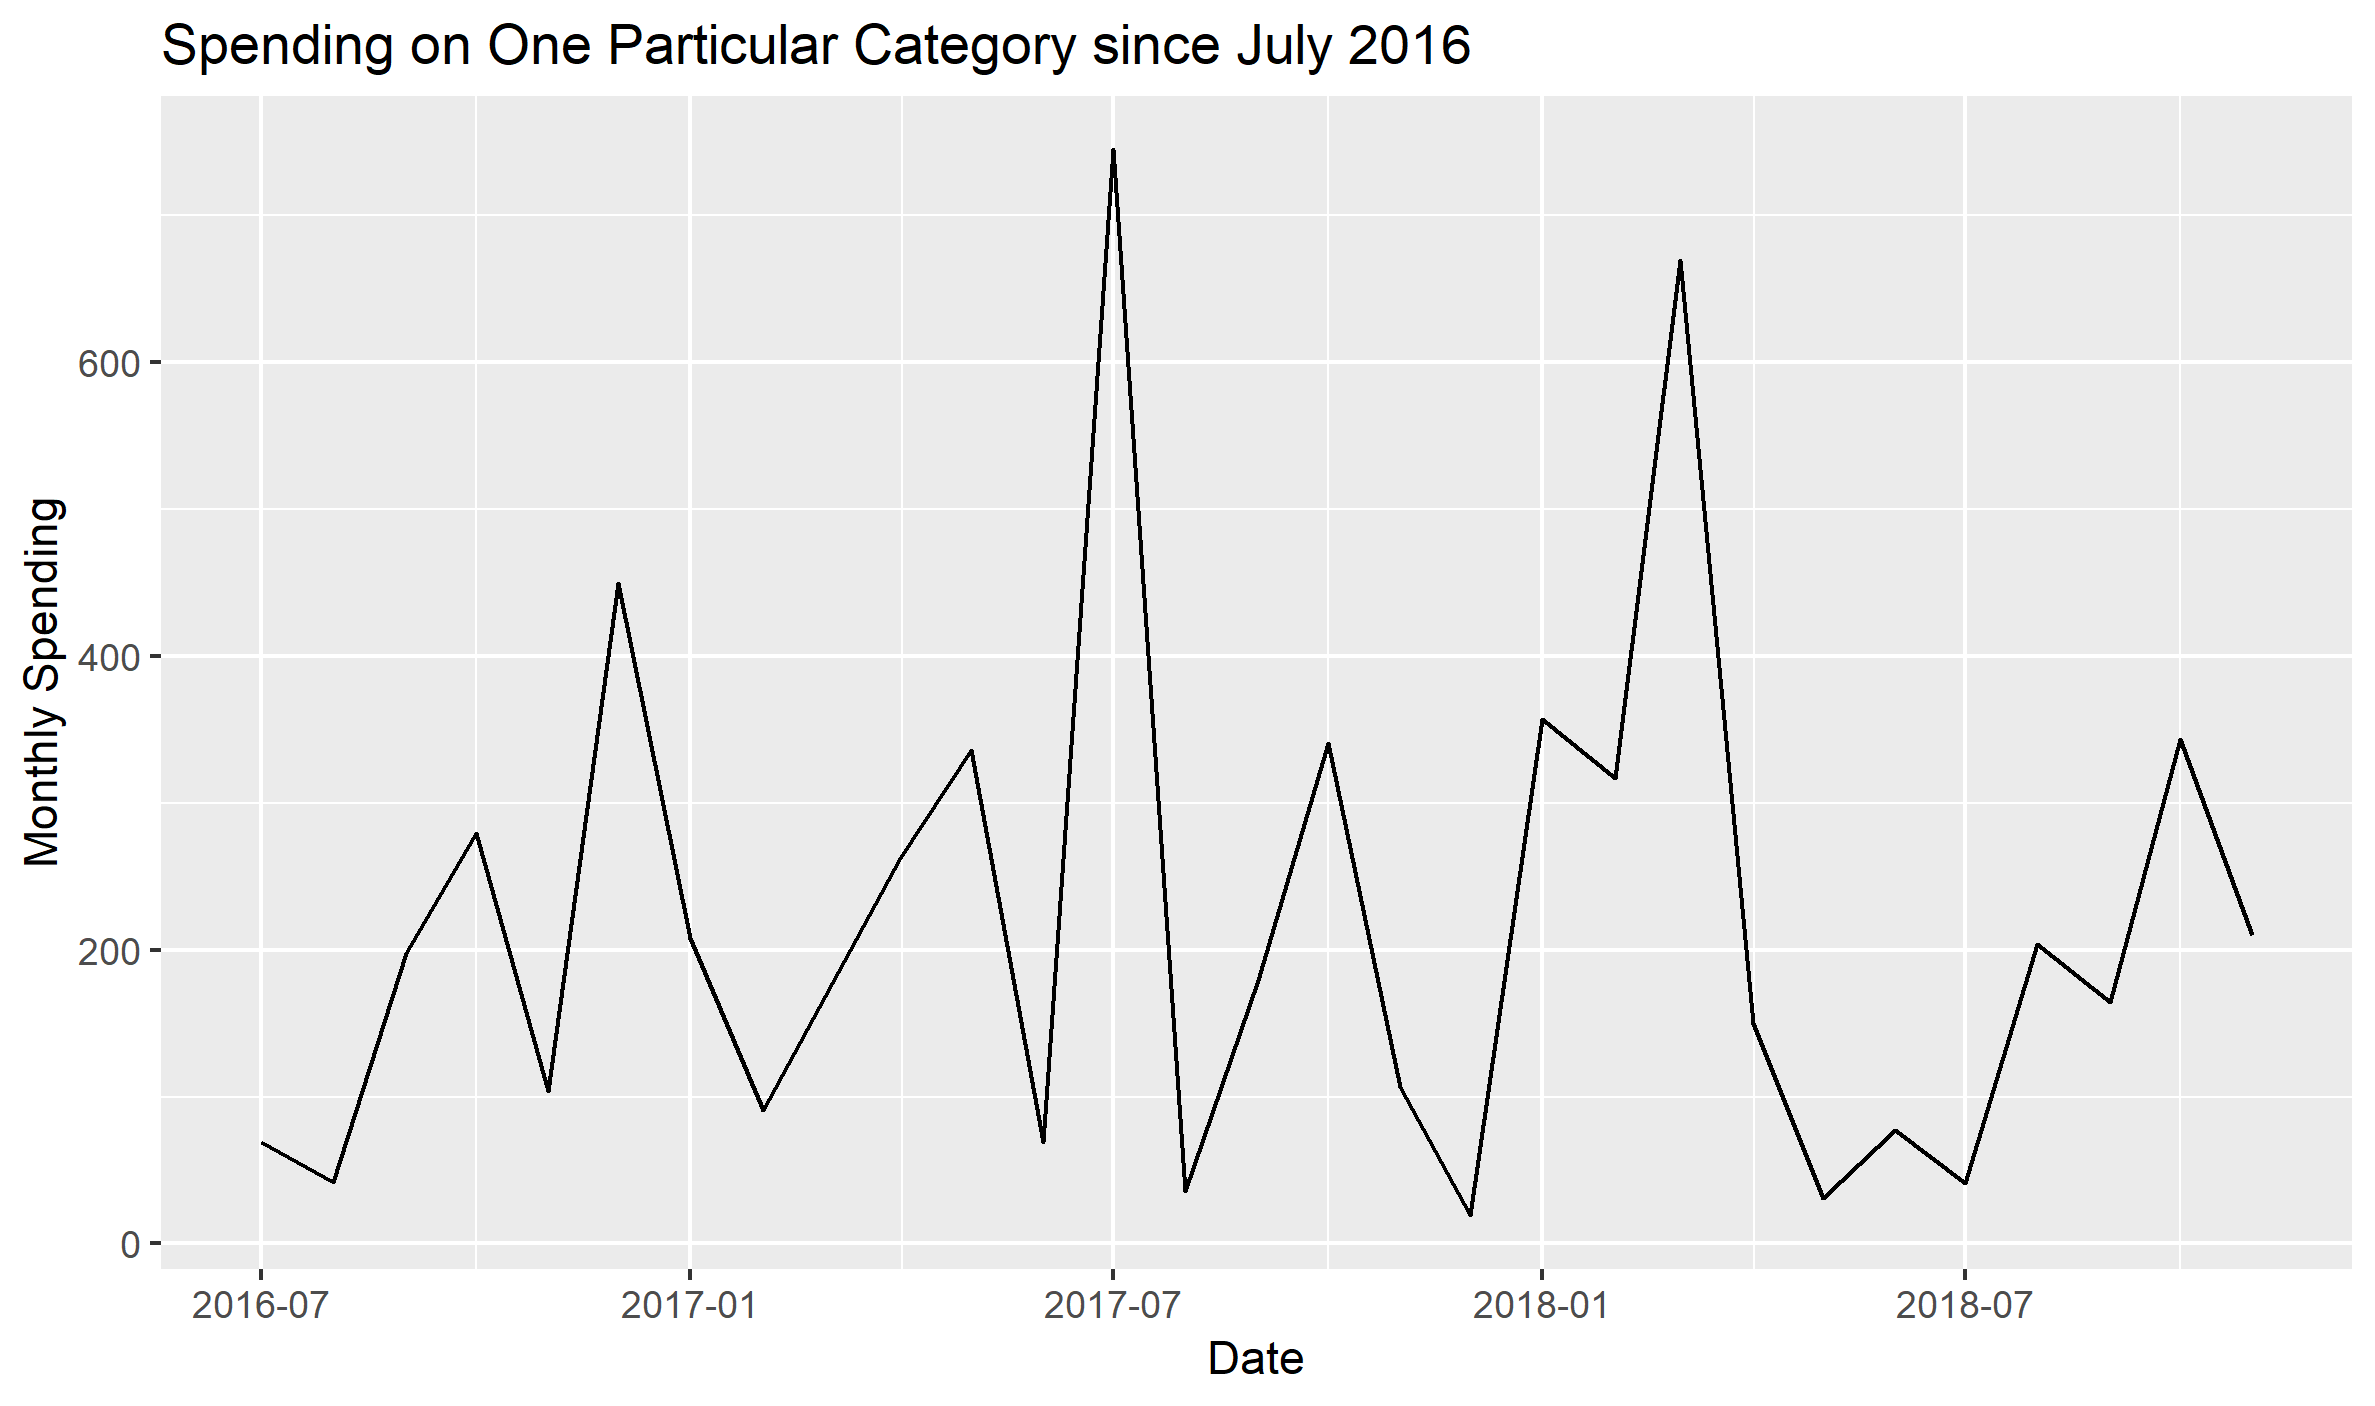
\includegraphics[width=0.7\linewidth]{../figures/Spending_Example}
		\caption{Monthly aggregation of spending for a particular category}
		\label{fig:spendingexample}
	\end{figure}
	
	
\end{updatematerial}


\section{Related Work} \label{sec:related_work}

There has been a lot of work on personal forecasting but most of it, to maintain simplicity, has been based off of using simple averages and running averages to predict the spending in the coming months. 

More advanced methods of prediction have, to my knowledge, never been used on personal financial data in this fashion before, and so I am to bring the more advanced analytical toolbox to the personal financial space in an effort to improve the forecasting accuracy and budgeting prediction. While methodologies are probably implemented in the private wealth space for ultra-high net worth clients, the people that need this prediction setup the most are the people who don't have the money to afford the inaccuracies that budgeting can allow in the first place. 

The prediction problem for time series is well studied however, and from that perspective there are a variety of methods that have been brought to the table. Anything from ARIMA modeling to Facebook's Prophet have been found to be useful. Gaussian Processes are something that may be useful to get variance estimates for each of the predictions, and other models that allow for smoothing of noisy data may be useful as well. ASAP, which we saw in class, is something that may be able to take out a large variety of the variation that financial data often brings about as well. 

\begin{updatematerial}
	In \cite{SVMFinance}, the authors used SVM, training on several properties of the time series up until this point, to predict how the stock will develop in the coming months. For this projects, I could use similar features such as volatility in the previous periods as well as skew and other technical oscillators borrowed from technical finance such as the Relative Strength Index and the Commodity Channel Index to use as training features and then run supervised machine learning algorithm on the data. In this way, I could hope to get away from the nature of the time-series modeling I have been doing in order to begin creeping into the more classical approaches to prediction treating the new monthly average as a predictive of the previous months. 
	
	In \cite{LongTail}, the authors used extreme-value modeling to come up with predictions of tail-risk in their financial modeling. Looking at my project from this lens, this is the measure that I am trying my hardest to estimate. Seeing as most people don't really care about the expected value of their spending, but rather would like to know the maximum for risk modeling, this paper actually may have changed my problem statement for some of the modeling a little bit. I would like to explore how to use these models to better estimate tail risk, and I want to build a model that is able to account for the tail risk of my spending. 
\end{updatematerial}


\section{Methodology} \label{sec:methodology}

Some of the methods that I plan to try for the forecasting piece of the assignment are as follows:
\begin{enumerate}
	\item As a baseline, how good / bad are running averages at predicting the future for financial data?
	\item ARIMA as a baseline
	\item Baysian Gaussian Processes as a means of modeling time series data with uncertainty estimates
	\item Baysian Hierarchal Modeling to predict the distributions of 1) the occurrence of a day with a particular type of spending. i.e. did I buy groceries today? and 2) if spending occurs, what is the distribution of the spending? i.e. I'm going to the grocery store, what am I going to spend?
	\item Facebook's Prophet - I've heard great things about the success of this system in predicting time series. I'm curious how well it will perform on the sparse data that I have
	\item Smoothing techniques like filtering - sometimes noise reduction allows one to see the forest through the trees - I'm hopeful that something like ASAP or DFT will allow the noise that is present in a time series to be reduced for financial data enough to make robust predictions. 
	\item Sequence processing such as a hidden Markov model may be very helpful as well and it is something that I would love to try
\end{enumerate}


Some of the methods that I plan to try for the metric piece of the assignment are as follows:
\begin{enumerate}
	\item Monthly Spending Index - at any given time, how much do I expect to spend in the next 30 days? This metric could be updated in real time to show an index of when I have been overspending or underspending
	\item Bullet charts to show good-caution-danger zone estimates for certain categories. Popularized by Stephen Few, these are great little charts and are highly dense information wise and can be very quickly made into a dashboard {\color{blue} \url{https://en.wikipedia.org/wiki/Bullet_graph}}
	\item Pain Index - Given the conjoint information from the beginning assessment, how likely are you to experience pain in the form of under-budgeting within the next month? Tracking this over time will let someone know how close they typically are to their goal and provide course correction in the event that they are unaware that they are not on track. 
\end{enumerate}

\begin{updatematerial}
	I plan to follow the methods plan that I have suggested above to identify which of the methods it the best at predicting financial data in the future. I would like to see how different methods compare and if I can gather anything out of the various methods by gaining predictive power or reducing the variance of the estimates. 
\end{updatematerial}


\section{Evaluation and Results} \label{sec:results}

From above: My evaluation metrics will include asymmetric L1 loss (the losses resulting from overprediction and a shortfall of money are far less severe than the losses resulting from foregone investment interest resulting from under budgeting and capital surplus). I want to run a conjoint analysis to determine what loss I can create that best aligns with how I experience loss. For this, I will place a large number of scenarios in front of myself and I want to evaluate which I would prefer in a given circumstance. For example, would I prefer to over budget by \$100 or would I prefer to under-budget vacation by \$80 and not be able to go out to dinner on the last night? Answers to questions such as these will be very useful in determining how I should assign loss measures and to which categories of my budget I should be the most focused on. 

In math, one such metric would be as follows (let $R$ be the realized amount of spending and $B$ be the amount Budgeted):
\begin{align}
Loss(R, B) &= w_1 \max(R - B, 0) \nonumber \\
&+ w_2 \max(B - R, 0)
\end{align}

Where, if $realized > budgeted$, then we have overspent and $w_1$ will drive our loss and the converse holds true for $w_2$. Given our discussion from before, it makes sense that $w_1 \geq w_2$ since the pain of having a shortfall, for most, will be greater than the gain that one experiences from optimizing their free cash flow. However, when I run the conjoint analysis, I hope to find out if this is really the case. 

The baseline metrics that I will use are both very common in the space:
\begin{enumerate}
	\item Running (or Simple) Average - Simple means and measures of center are the most common implementation for many of the prediction metrics from month to month. This is the method that is used in my budgeting program currently, and its inadequacy is the main reason why I thought of this project. 
	\item ARIMA - this is probably the most sophisticated model that most anyone who works with basic financial data uses since it is widely implemented and this is usually the most advanced (and only) mention of time series in most business schools\footnote{During my time in Ross, this was only mentioned in an advanced analytics course at the 400 level and was a highly non-standard part of the curriculum. During my time in banking, most forecasting was done at a far more micro level using correlations and so large scale time series analysis were left to the research economists who used mean expectation algorithms for stability.}. 
\end{enumerate}

\begin{updatematerial}
	Looking at the Baseline models, there is still lots of improvement to do to determine how the models will perform, but with an $L_1$ loss all above 150, I think that the unweighted mean and the ARIMA models are going to be good baselines to begin with. I have carried out the following baseline models with their results:
	\begin{itemize}
		\item Basic lagging mean: This method used the running equal-weight mean with lag periods 1:15. If $lookback = 0$, this is equivalent to using the previous month's value to predict this months value, and a lag of fifteen would use the average from the previous fifteen months to predict this month. The error is printed out in terms of the average $L_1$ error that each method produced. See figure  \ref{fig:laggedmeanpredictionresults} for the visualization of the errors
		% latex table generated in R 3.4.3 by xtable 1.8-2 package
		% Mon Nov 12 22:16:16 2018
		\begin{table}[ht]
			\centering
			\begin{tabular}{rlr}
				\hline
				& Type & error \\ 
				\hline
				1 & Mean(lookback = 0) & 225.68 \\ 
				2 & Mean(lookback = 1) & 203.28 \\ 
				3 & Mean(lookback = 2) & 183.10 \\ 
				4 & Mean(lookback = 3) & 191.36 \\ 
				5 & Mean(lookback = 4) & 184.09 \\ 
				6 & Mean(lookback = 5) & 170.71 \\ 
				7 & Mean(lookback = 6) & 168.43 \\ 
				8 & Mean(lookback = 7) & 160.13 \\ 
				9 & Mean(lookback = 8) & 157.74 \\ 
				10 & Mean(lookback = 9) & 160.21 \\ 
				11 & Mean(lookback = 10) & 160.86 \\ 
				12 & Mean(lookback = 11) & 159.83 \\ 
				13 & Mean(lookback = 12) & 159.31 \\ 
				14 & Mean(lookback = 13) & 159.76 \\ 
				15 & Mean(lookback = 14) & 157.38 \\ 
				16 & Mean(lookback = 15) & 158.63 \\ 
				\hline
			\end{tabular}
		\end{table}
		We can see that the highest lags had the lowest errors
		\item ARIMA Modeling: The ARIMA error is expressed in Figure \ref{fig:arimamodelingerrorinit}. We can see that the simplest model (one without a linear trend or seasonality)  has the lowest error on the chosen problem
	\end{itemize}
	Expansions on this, to be implemented shortly, include different time period aggregations (maybe weekly) or to use other methods of predicting the outflows in a month (Monte Carlo or other ensemble methods to build up months one day at a time. )
\end{updatematerial}
\begin{figure}
	\centering
	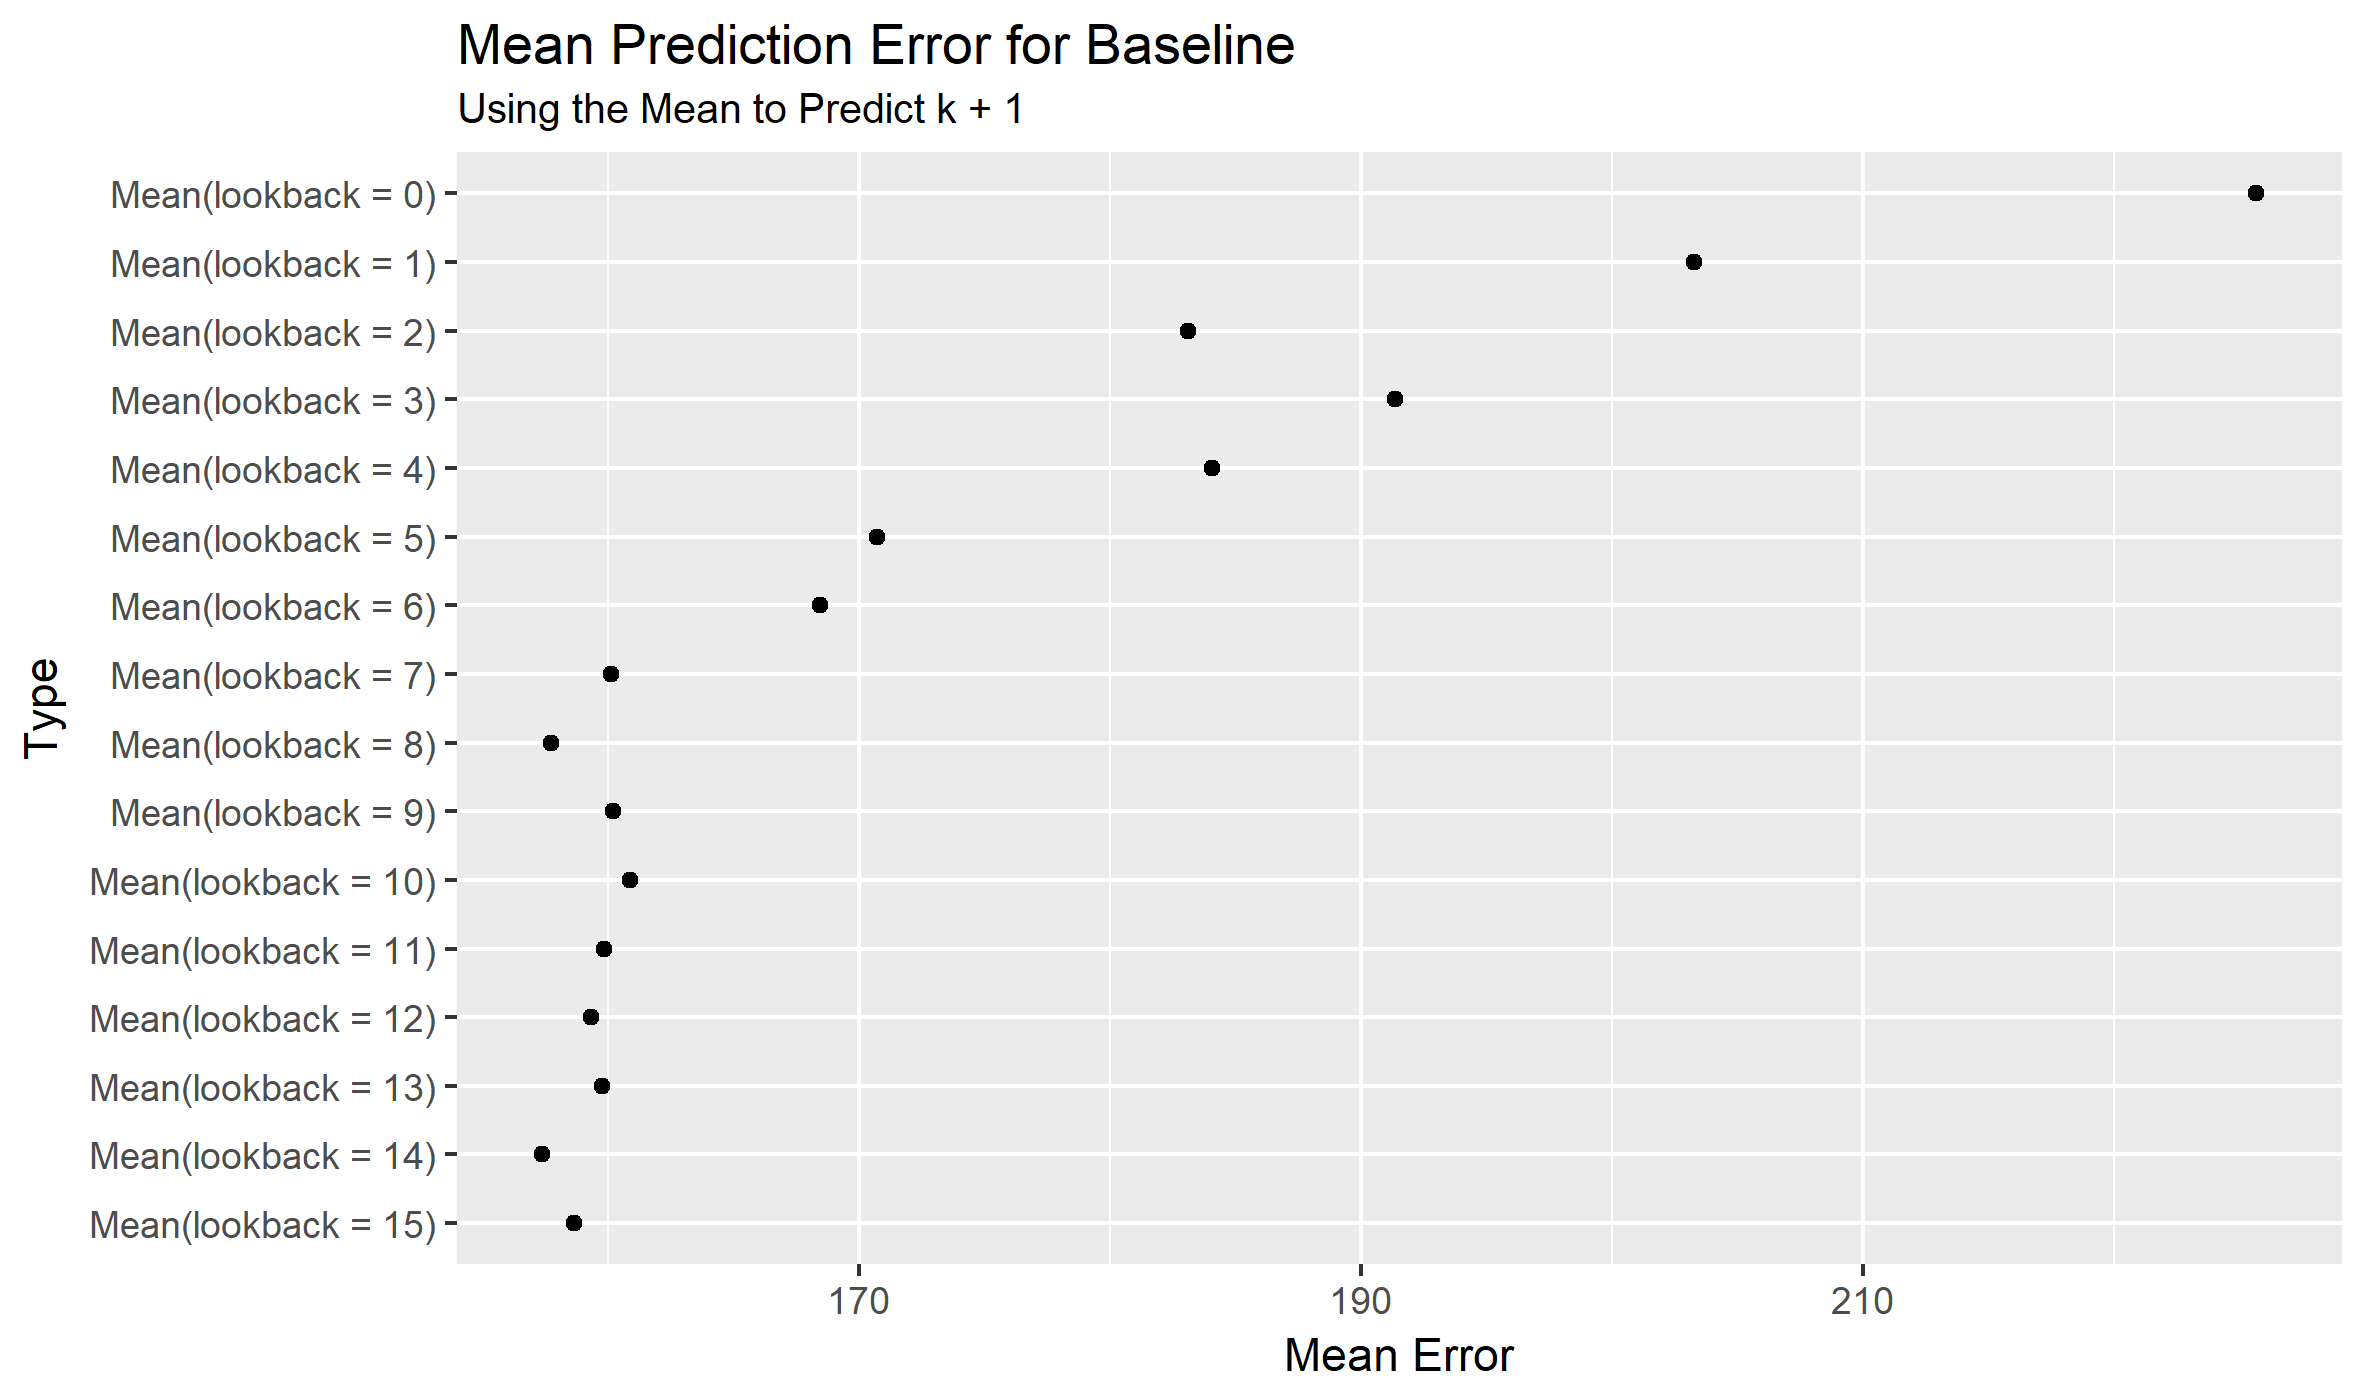
\includegraphics[width=1\linewidth]{../figures/Lagged_Mean_Prediction_Results}
	\caption{Average $L_1$ error for the lagged mean models}
	\label{fig:laggedmeanpredictionresults}
\end{figure}
\begin{figure}
	\centering
	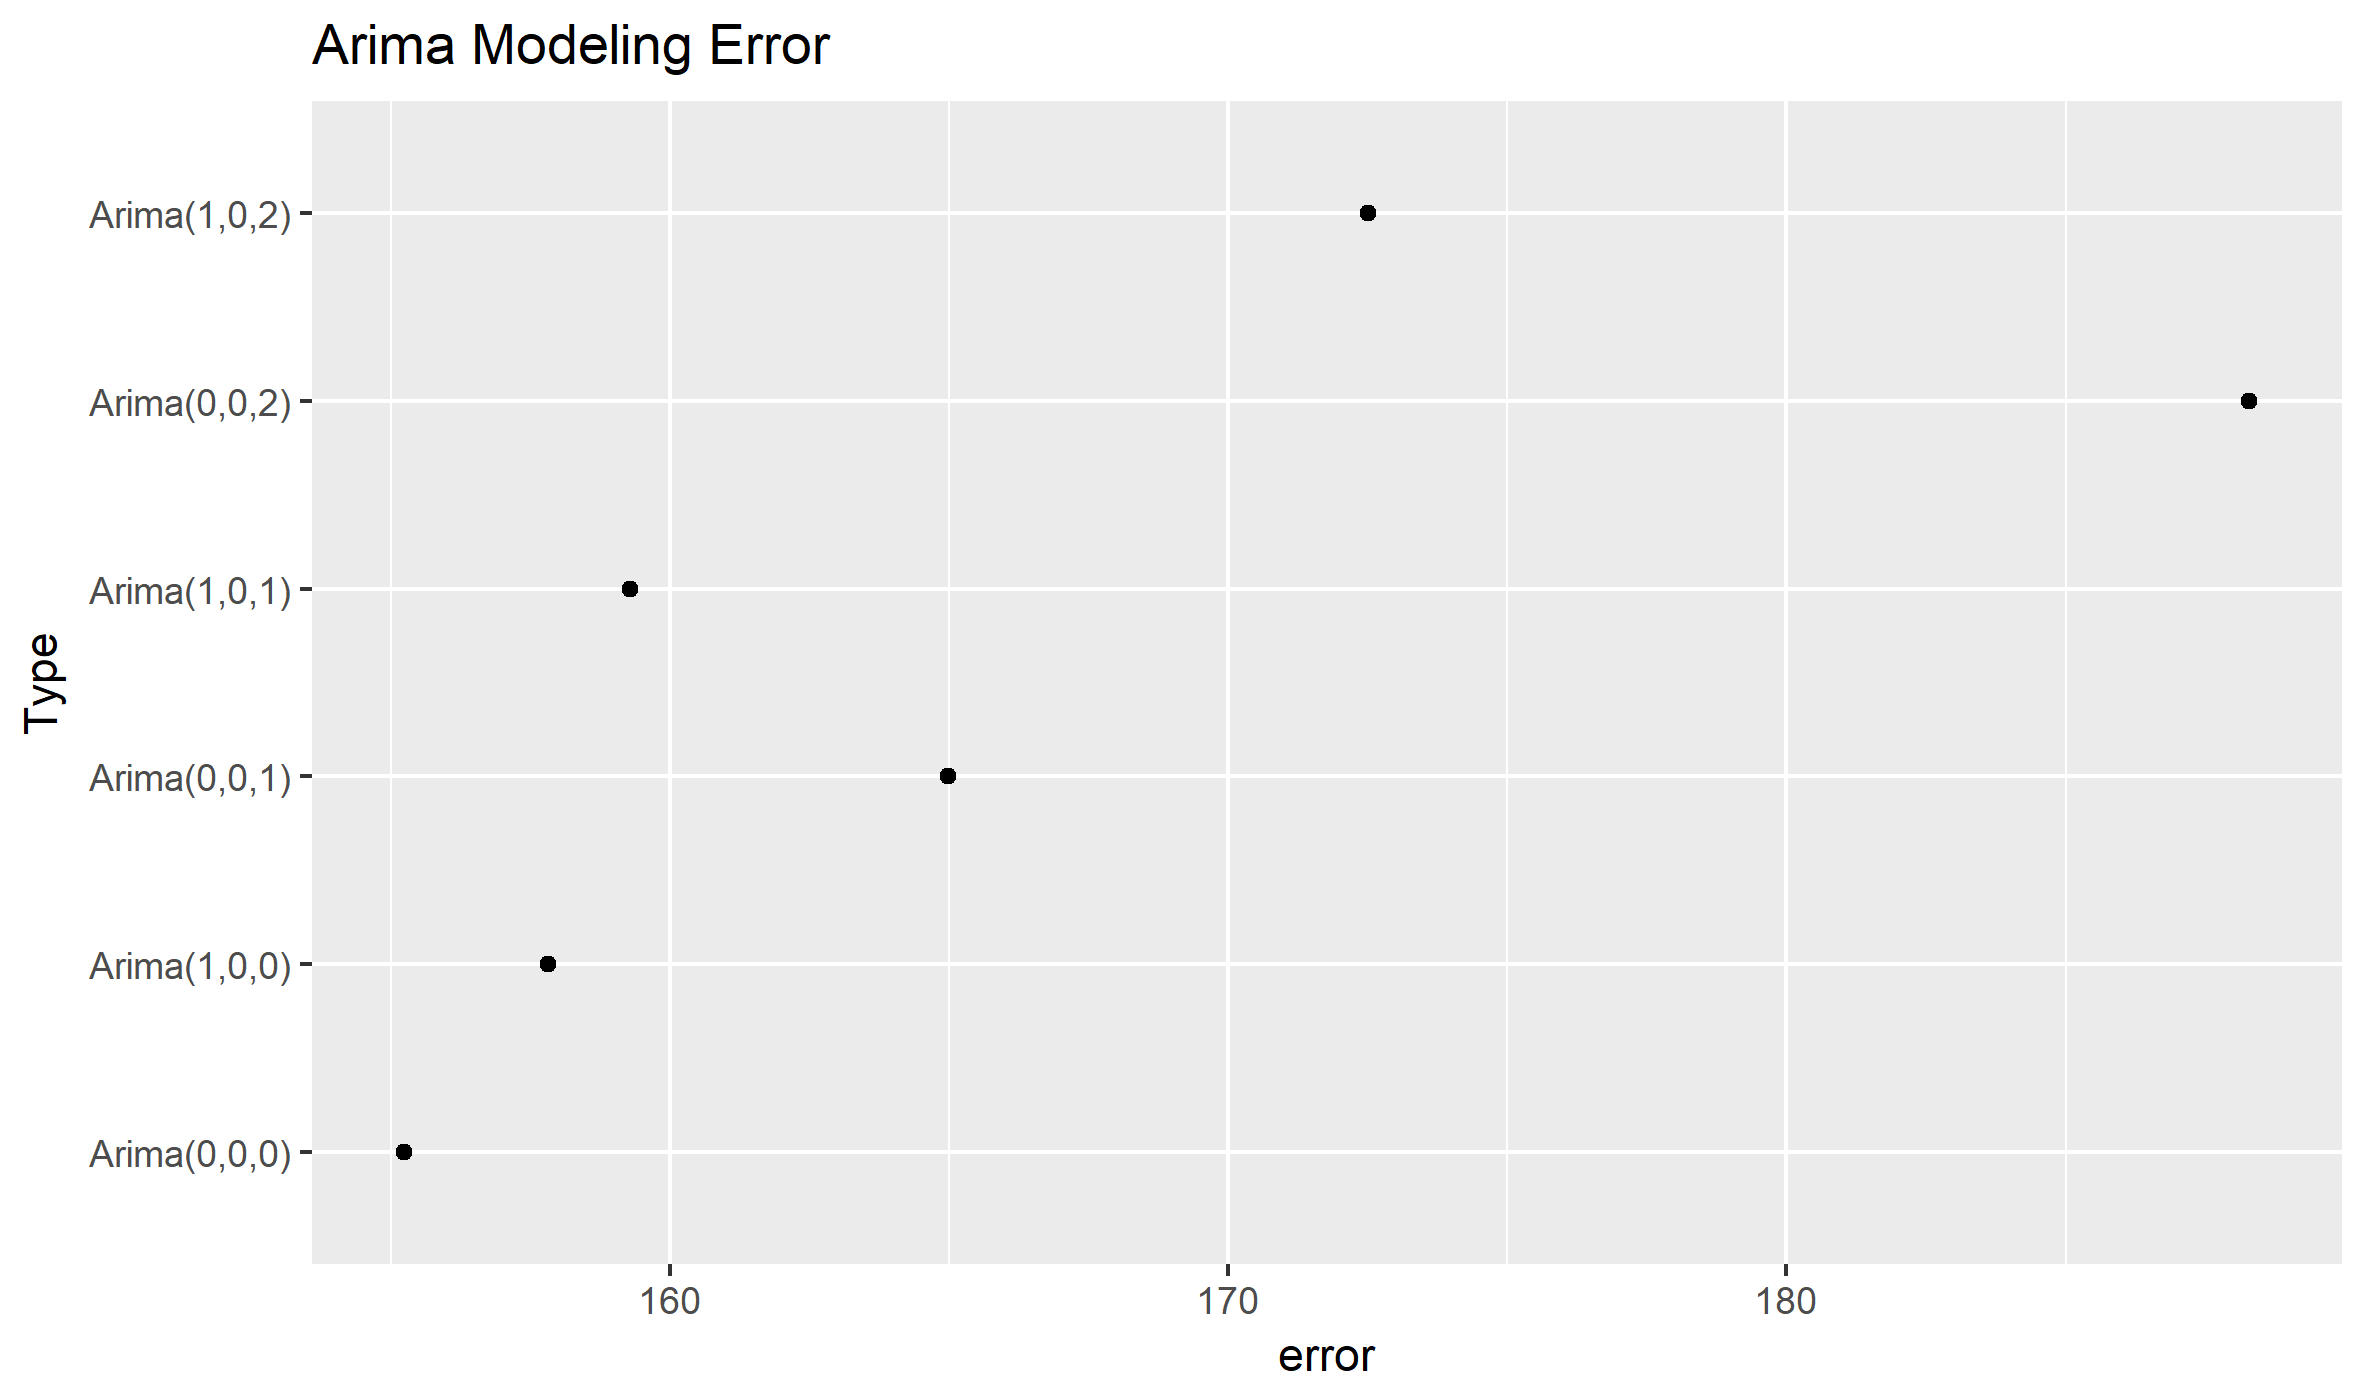
\includegraphics[width=1\linewidth]{../figures/Arima_Modeling_Error_Init}
	\caption{Anova Error for R Present Models}
	\label{fig:arimamodelingerrorinit}
\end{figure}




%This section provides an overview of how you evaluated your method on the data.  What methods did you compare against?  How successful were you?  Describe the exact evaluation setup and what kinds of
%steps were taken.

%You should also clearly define some baselines to compare your system against.
%One baseline should be random performance.  A second baseline should be
%something reasonable that doesn't require much knowledge or learning.  For example, if you're doing a recommendation engine, always choosing the average rating is a useful baseline.

%\textbf{ \color{red} For the proposal, you should propose a very simple baseline to compare your model against and a description of the evaluation metric(s) you intent to use.  You \textit{must} include this baseline description for credit, as it is critical to  proposing an evaluatable data mining task.}

%
%\begin{figure}
%\centering
%% Note: text width is the width of both columns
%%\includegraphics[width=0.38\textwidth]{examplefigure.pdf}
%\caption{Eventually, you'll have cool figures to show here.}
%\end{figure}

\section{Discussion}



%The discussion section is where you start to unpack the results for the reader
%to help them understand what was learned.  You may not have many results at the
%moment (but you should have some!) so you can discuss here what has gone wrong
%and right in your current setup.  For example, maybe you realized you needed
%more data, or maybe you realized that the SVD was not helping your analysis.
%The discussion should point the way to what work will be done next.


%\textbf{ \color{red} You can leave this section blank. }

\begin{updatematerial}
	With an average error for the simple mean calculation of over 150 and over 160 for the best ARIMA model, the baseline performs rather poorly but this is something that I think that could be useful for measuring the success of future methods. In short, if you ran this model, and asked it what you would spend in the next month, it would give you an estimate with an average $L_1$ error of \$150 which tells us that if it predicts \$400 in spending on food, that the error bars are from \$100 to \$700 which make the estimates next to useless. 
	
	This is a good baseline to begin off of, because it tells us that the mean function of the past data is not the most important thing in predicting this data on a pure-monthly basis, and this tells us that methods will inherently need to work with more granular aggregations (which are possible since I have the daily data) in order to gain useful insights into the modeling of the expected value. 
\end{updatematerial}





\section{Work Plan}

My plan for this project roughly follows the following guideline:
\begin{enumerate}
	\item Gather the data from my budgeting program. I already have a workflow for this
	\begin{updatematerial}
		This has been completed
	\end{updatematerial}
	\item Determine which categories are worth modeling - I'm looking at any variable expenses as being the most useful thing to model. Fixed expenses like rent are contractual and can be modeled statically
	\begin{updatematerial}
		I have decided to spend most of my time modeling categories like ``Spending money'' which is a catch-all for random things like house supplies and school materials and ``Food and Drinks'' which includes every single meal that I have eaten out that does not include the meals that I make with my own groceries as well as ``Groceries'' which is my tracking of my grocery expenditures.
	\end{updatematerial}
	\item Begin building look-ahead prediction models and comparing them. 
	\begin{enumerate}
		\item Start with base models. Assess prediction accuracy
		\begin{updatematerial}
			This has been implemented as of this writing using the baseline for the means as well as the ARIMA model
		\end{updatematerial}
		\item Work up to more advanced models
		\item Try to combine results using stacking to improve prediction error 
		\begin{updatematerial}
			I don't think that this step will happen due to the modeling complexity already
		\end{updatematerial}
		\item Reduce data-size as much as possible to see how much data we need for ``good enough'' accuracy
		\begin{updatematerial}
			This is an implicit part of the error analysis and will probably be included as a result
		\end{updatematerial}
	\end{enumerate}
	\item Begin looking at metrics that assess the health of a persons spending as a means of visualizing progress. 
		\begin{updatematerial}
			This is the part of the project that is the most TBD due to the fact that the timing is going to be quite intensive to model out all of the other parts and get the performance of the models where I would like to. This, I think, is the most useful part of the project though for my purposes and it is something that I would like to focus on if I get the time. 
		\end{updatematerial}
	\begin{enumerate}
		\item Track financial ratios and see if they are ``useful''
		\item Look at smoothing procedures to see if they add information
		\item Look at simulation based visualizations to see if they add anything interesting
	\end{enumerate}
\end{enumerate}

%\textbf{ \color{red}  Normally, you would have a conclusion to end the work, but as this is a project proposal,
%you'll end with a plan for how you'll accomplish your project.  We hope this section can help you think at a high-level about which tasks are necessary to get to the point where you have a working model.  Of course, plans are often made and then changed when new information or challenges emerge, so we won't hold you you to this.  However, the act of writing a plan can greatly help you figure out how think about the process and, in general, projects that are proposed with more concrete work plans tend to be more successful.
%}

%\section{Multi-person Team Justification}
%
%\textbf{ \color{red} If you have more than one person on your project, you should justify why the work requires the number of people you have.  In addition, you should provide a concrete explanation of what each team member is expected to do, keeping in mind that all team members need to be doing \textit{some} kind of data mining for the project.}

\section*{Acknowledgments}

My brother, an accountant, and I as well as several friends have discussed beginning a financial advisory firm focusing on tax arbitrage and investing advice based on tailored risk analysis. My background in finance and financial modeling heavily informs my views of financial predictions in general, and I know how noisy the real world is with this kind of data. Having always been interested in personal finance, this aspect of modeling out my finances is something I have attempted in the past using various simulation based methods, but I have never taken a deep dive into quantifying error nor coming up with a system for prediction and analysis. I hope to expand this for the ambitions of a past self and for the benefit of a potential business

%If you got help from anyone or had substantive discussions, please acknowledge
%those people here and describe how they contributed.  The work you do for your
%project should be entirely your own.

% include your own bib file like this:
%\bibliography{references}
%\bibliographystyle{acl_natbib}

%\textbf{\color{red} Note that you must cite all your references, e.g., \cite{wang2014studentlife}}

%\appendix

%\begin{thebibliography}{9}
%	
%	\bibitem{BNP} 
%	BNP Paribas - During my time at BNP Paribas in New York, this was often a statistic that was used in client meetings and for presentations. 
%	
%	\bibitem{SVMFinance}
%	Kim, Kyoung-jae. “Financial Time Series Forecasting Using Support Vector Machines.” NeuroImage, Academic Press, 13 May 2003, www.sciencedirect.com/science/article/pii/S0925231203003722\#SEC3.
%	
%	\bibitem{LongTail}
%	McNeil, Alexander. “Estimation of Tail-Related Risk Measures for Heteroscedastic Financial Time Series: an Extreme Value Approach.” NeuroImage, Academic Press, 1 Dec. 2000, www.sciencedirect.com/science/article/pii/S0927539800000128.
%	
%\end{thebibliography}


%\section{Supplemental Material}
%\label{sec:supplemental}
%
%If you want to put longer examples of data and code, put it here in the appendix.  

\end{document}
